\documentclass[border=10pt]{standalone}
\usepackage[svgnames]{xcolor}
\usepackage{amsmath}
\usepackage{pgfplots}
\pgfplotsset{compat=newest}
\usepackage[sfdefault]{FiraSans}
\usepackage{FiraMono}
\renewcommand*\familydefault{\sfdefault}
\begin{document}
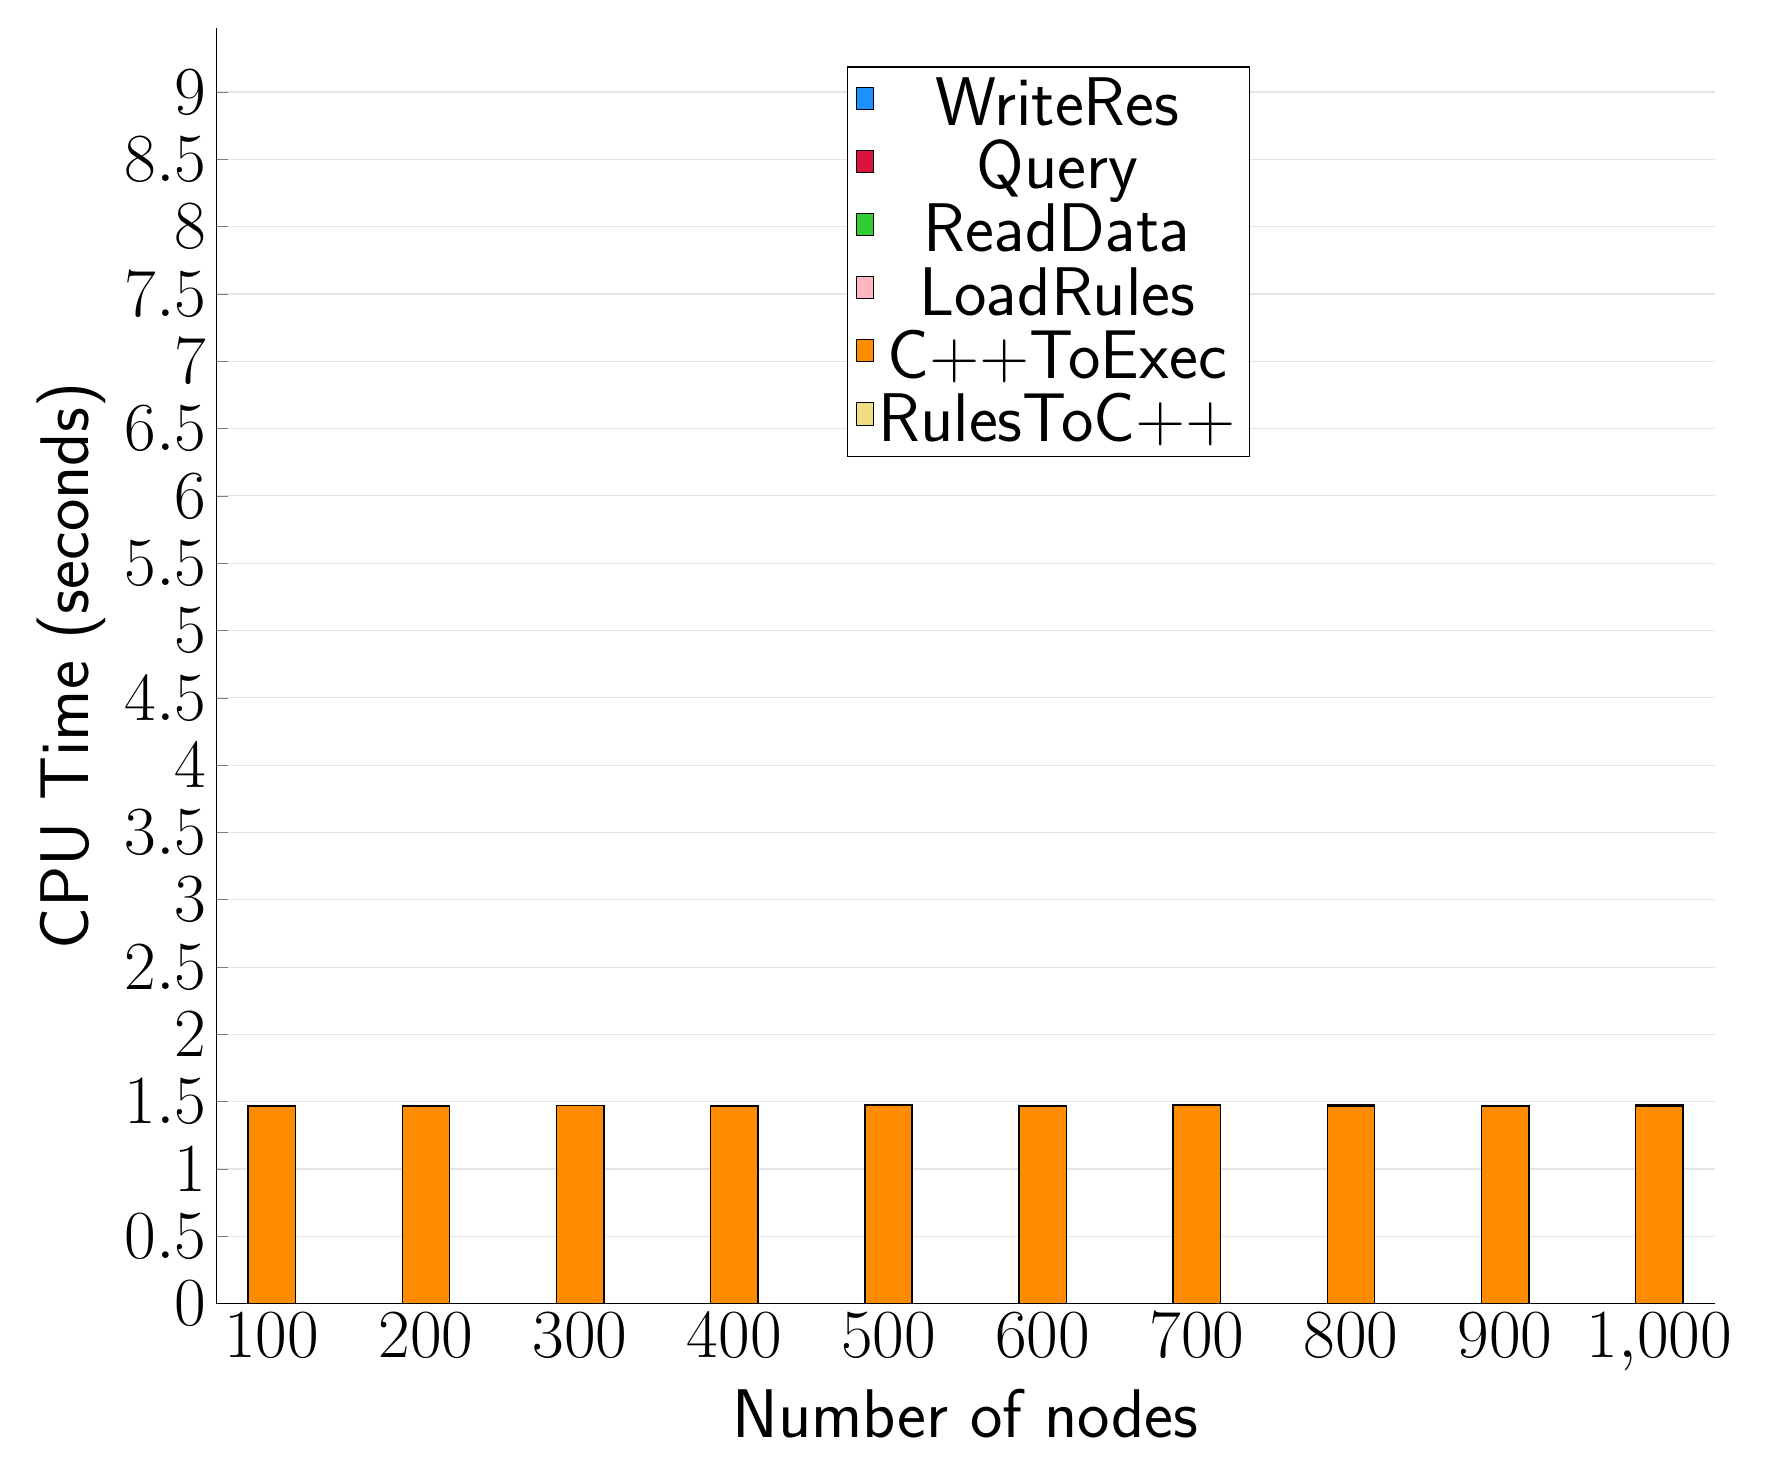
\begin{tikzpicture}
\begin{axis}[
   ybar stacked,
   width=1.7\textwidth,
   bar width=0.6cm,
   ymajorgrids, tick align=inside,
   major grid style={draw=gray!20},
   xtick=data,
   ymin=0, ymax=9.474,
   axis x line*=bottom,
   axis y line*=left,
   enlarge x limits=0.04,
   legend style={
       at={(0.69, 0.97)},
       anchor=north east,
       legend columns=1,
       font=\Huge,
   },
   ylabel={CPU Time (seconds)},
   xlabel={Number of nodes},
   label style={font=\Huge},
   tick label style={font=\Huge},
]
\addlegendimage{fill=DodgerBlue, draw=black, line width=0.2pt}
\addlegendentry{WriteRes}
\addlegendimage{fill=Crimson, draw=black, line width=0.2pt}
\addlegendentry{Query}
\addlegendimage{fill=LimeGreen, draw=black, line width=0.2pt}
\addlegendentry{ReadData}
\addlegendimage{fill=LightPink, draw=black, line width=0.2pt}
\addlegendentry{LoadRules}
\addlegendimage{fill=DarkOrange, draw=black, line width=0.2pt}
\addlegendentry{C++ToExec}
\addlegendimage{fill=LightGoldenrod, draw=black, line width=0.2pt}
\addlegendentry{RulesToC++}
\addplot +[fill=LightGoldenrod, draw=black, line width=0.55pt] coordinates {
(100, 0.0020000000000000005)
(200, 0.0)
(300, 0.0)
(400, 0.0)
(500, 0.0)
(600, 0.0)
(700, 0.0)
(800, 0.0)
(900, 0.0)
(1000, 0.0)
};
\addplot +[fill=DarkOrange, draw=black, line width=0.55pt] coordinates {
(100, 1.466)
(200, 1.4659999999999997)
(300, 1.47)
(400, 1.468)
(500, 1.47)
(600, 1.4659999999999997)
(700, 1.472)
(800, 1.468)
(900, 1.466)
(1000, 1.468)
};
\addplot +[fill=LightPink, draw=black, line width=0.55pt] coordinates {
(100, 0.0001518)
(200, 0.00017400000000000003)
(300, 0.00017999999999999998)
(400, 0.0001578)
(500, 0.0001672)
(600, 0.00016680000000000002)
(700, 0.0001698)
(800, 0.00017120000000000001)
(900, 0.0001604)
(1000, 0.0001714)
};
\addplot +[fill=LimeGreen, draw=black, line width=0.55pt] coordinates {
(100, 0.0007472)
(200, 0.0012092000000000001)
(300, 0.0013594000000000002)
(400, 0.0018966)
(500, 0.0021666)
(600, 0.0025721999999999997)
(700, 0.0030719999999999996)
(800, 0.0032824000000000004)
(900, 0.0035574)
(1000, 0.0039148)
};
\addplot +[fill=Crimson, draw=black, line width=0.55pt] coordinates {
(100, 0.0001658)
(200, 0.00038580000000000005)
(300, 0.0004724)
(400, 0.0006514)
(500, 0.0008289999999999999)
(600, 0.0009808)
(700, 0.0012016000000000002)
(800, 0.0012864)
(900, 0.0013732)
(1000, 0.0017209999999999999)
};
\addplot +[fill=DodgerBlue, draw=black, line width=0.55pt] coordinates {
(100, 0.00042239999999999997)
(200, 0.0006124)
(300, 0.0006018)
(400, 0.0007562000000000001)
(500, 0.000775)
(600, 0.0009381999999999999)
(700, 0.0010148000000000002)
(800, 0.0010573999999999998)
(900, 0.0010078)
(1000, 0.0010332)
};
\end{axis}
\end{tikzpicture}

\end{document}
